
\documentclass[border=10pt]{standalone}
\usepackage[table]{xcolor}
\usepackage{amsmath,amssymb,amsfonts,mathtools,bm}
\usepackage{booktabs,array}
\usepackage{tikz}
\usetikzlibrary{arrows.meta,positioning,calc,backgrounds,fit,shapes.geometric,decorations.pathreplacing}
\usepackage{pgfplots}
\pgfplotsset{compat=1.18}
\definecolor{sbnavy}{HTML}{1A2A4F}
\definecolor{sbteal}{HTML}{1C7293}
\definecolor{sbaccent}{HTML}{B5651D}
\definecolor{sbgrey}{HTML}{8A94A6}
\definecolor{sblight}{HTML}{EAF1F5}
\newcommand{\cmark}{\textcolor{sbteal}{\ensuremath{\boldsymbol{\checkmark}}}}
\newcommand{\xmark}{\textcolor{sbgrey}{\ensuremath{\boldsymbol{\times}}}}
\newcommand{\eqcol}{\color{sbnavy}}
\begin{document}
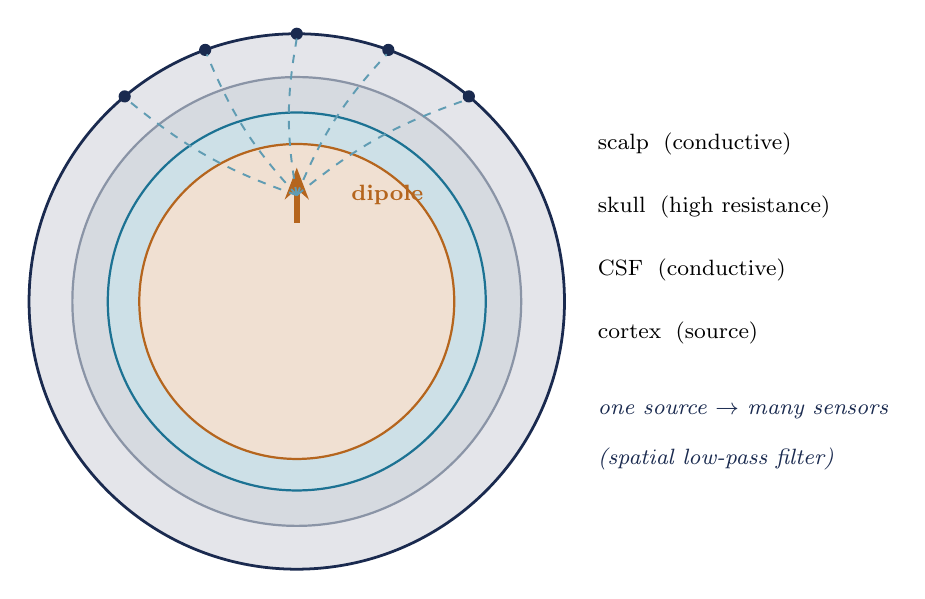
\begin{tikzpicture}[font=\sffamily]
  \foreach \r/\col/\lab/\sig in {3.4/sbnavy!12/scalp/{\footnotesize scalp}, 2.85/sbgrey!35/skull/{\footnotesize skull (insulator)}, 2.4/sbteal!22/CSF/{\footnotesize CSF}, 2.0/sbaccent!20/cortex/{\footnotesize cortex}}{
     \fill[\col] (0,0) circle (\r);
  }
  \draw[sbnavy,line width=1pt] (0,0) circle (3.4);
  \draw[sbgrey,line width=0.8pt] (0,0) circle (2.85);
  \draw[sbteal,line width=0.8pt] (0,0) circle (2.4);
  \draw[sbaccent,line width=0.8pt] (0,0) circle (2.0);
  % dipole source
  \draw[-{Stealth[length=4mm]},sbaccent,line width=2pt] (0,1.0) -- (0,1.7);
  \node[sbaccent,font=\footnotesize\bfseries] at (1.15,1.35) {dipole};
  % electrodes on scalp (top arc)
  \foreach \a in {50,70,90,110,130}{
     \fill[sbnavy] (\a:3.4) circle (2.2pt);
  }
  % smeared spread (dashed) from dipole to several electrodes
  \foreach \a in {50,70,90,110,130}{
     \draw[sbteal!70,dashed,line width=0.7pt] (0,1.35) to[bend left=10] (\a:3.34);
  }
  % labels at right
  \node[anchor=west,font=\footnotesize] at (3.7,2.0)  {scalp \;(conductive)};
  \node[anchor=west,font=\footnotesize] at (3.7,1.2)  {skull \;(high resistance)};
  \node[anchor=west,font=\footnotesize] at (3.7,0.4)  {CSF \;(conductive)};
  \node[anchor=west,font=\footnotesize] at (3.7,-0.4) {cortex \;(source)};
  \node[anchor=west,font=\footnotesize\itshape,text=sbnavy] at (3.7,-1.4) {one source $\rightarrow$ many sensors};
  \node[anchor=west,font=\footnotesize\itshape,text=sbnavy] at (3.7,-2.0) {(spatial low-pass filter)};
\end{tikzpicture}
\end{document}